%%%%%%%%%%%%%%%%%%%%%%%%%%%%%%%%%%%%%%%%%
% Programming/Coding Assignment
% LaTeX Template
%
% This template has been downloaded from:
% http://www.latextemplates.com
%
% Original author:
% Ted Pavlic (http://www.tedpavlic.com)
%
% Note:
% The \lipsum[#] commands throughout this template generate dummy text
% to fill the template out. These commands should all be removed when
% writing assignment content.
%
% This template uses a Perl script as an example snippet of code, most other
% languages are also usable. Configure them in the "CODE INCLUSION
% CONFIGURATION" section.
%
%%%%%%%%%%%%%%%%%%%%%%%%%%%%%%%%%%%%%%%%%

%----------------------------------------------------------------------------------------
% PACKAGES AND OTHER DOCUMENT CONFIGURATIONS
%----------------------------------------------------------------------------------------

\documentclass{scrartcl}

\usepackage[T1]{fontenc}
\usepackage[utf8x]{inputenc}

\usepackage{fancyhdr} % Required for custom headers
\usepackage{lastpage} % Required to determine the last page for the footer
\usepackage{extramarks} % Required for headers and footers
\usepackage[usenames,dvipsnames]{color} % Required for custom colors
\usepackage{graphicx} % Required to insert images
\usepackage{listings} % Required for insertion of code
\usepackage{courier} % Required for the courier font

\usepackage{hyperref}

\linespread{1.1} % Line spacing

% Set up the header and footer
\pagestyle{fancy}
\lhead{\hmwkAuthorName \\} % Top left header
\chead{\hmwkClass: \hmwkTitle} % Top center head
\rhead{\firstxmark} % Top right header
\lfoot{\lastxmark} % Bottom left footer
\cfoot{} % Bottom center footer
\rfoot{Page\ \thepage\ of\ \protect\pageref{LastPage}} % Bottom right footer
\renewcommand\headrulewidth{0.4pt} % Size of the header rule
\renewcommand\footrulewidth{0.4pt} % Size of the footer rule

\setlength\parindent{0pt} % Removes all indentation from paragraphs

%----------------------------------------------------------------------------------------
%	CODE LISTINGS SETUP
%----------------------------------------------------------------------------------------
\usepackage{color}
\usepackage[usenames,dvipsnames,svgnames,table]{xcolor}
\colorlet{MAROON}{Maroon}
\usepackage{minted}
\providecommand*{\listingautorefname}{Listing}

%----------------------------------------------------------------------------------------
% NAME AND CLASS SECTION
%----------------------------------------------------------------------------------------

\newcommand{\hmwkTitle}{Project 3 -- Particle Swarm Optimization} % Assignment title
\newcommand{\hmwkDueDate}{Wednesday,\ Novemeber\ 24,\ 2013} % Due date
\newcommand{\hmwkClass}{IT3105} % Course/class
\newcommand{\hmwkClassTime}{} % Class/lecture time
\newcommand{\hmwkClassInstructor}{Lecturer: Jo Skjermo, Keith Downing} % Teacher/lecturer
\newcommand{\hmwkAuthorName}{Pablo Liste Garcia \& Dominik Horb} % Your name


\usepackage{tabularx}
%----------------------------------------------------------------------------------------
% TITLE PAGE
%----------------------------------------------------------------------------------------

\title{
\vspace{2in}
\textmd{\textbf{\hmwkClass:\ \hmwkTitle}}\\
\normalsize\vspace{0.1in}\small{Due\ on\ \hmwkDueDate}\\
\vspace{0.1in}\large{\textit{\hmwkClassInstructor\ \hmwkClassTime}}
\vspace{3in}
}

\author{\textbf{\hmwkAuthorName}}
\date{} % Insert date here if you want it to appear below your name

%----------------------------------------------------------------------------------------

\begin{document}

\maketitle

%----------------------------------------------------------------------------------------
% TABLE OF CONTENTS
%----------------------------------------------------------------------------------------

%\setcounter{tocdepth}{1} % Uncomment this line if you don't want subsections listed in the ToC

\newpage
\tableofcontents
\newpage

\section{Architecture Description}

The idea for the architecture of the system we devised was to have generalized Particles that would be able to store solutions to very different kinds of constraint based problems and a basic \textit{ParticleSwarm} class, that would hold similarities between the different implementations.

The hardest part for us to understand was the difference between binary particles and ones that could hold floating point solutions and how the vectors could be used to represent the solutions to the given problems. As we were just able to implement the PSO for the Knapsack problem due to time constraints, we couldn't test how the general structure we have would hold up to cater to more different problem styles. The system architecture would probably need some more tweaking, we however believe, that it goes in the right direction to be very versatile.

\section{Task 3 -- Simple Knapsack Problem}

As you can see in \autoref{fig:simple-knapsack-output}, the number of packages in a solution that is found by our implementation is usually around 30 with the highest fitness going slightly above 200 during good runs.

\begin{figure}[!htbp]
 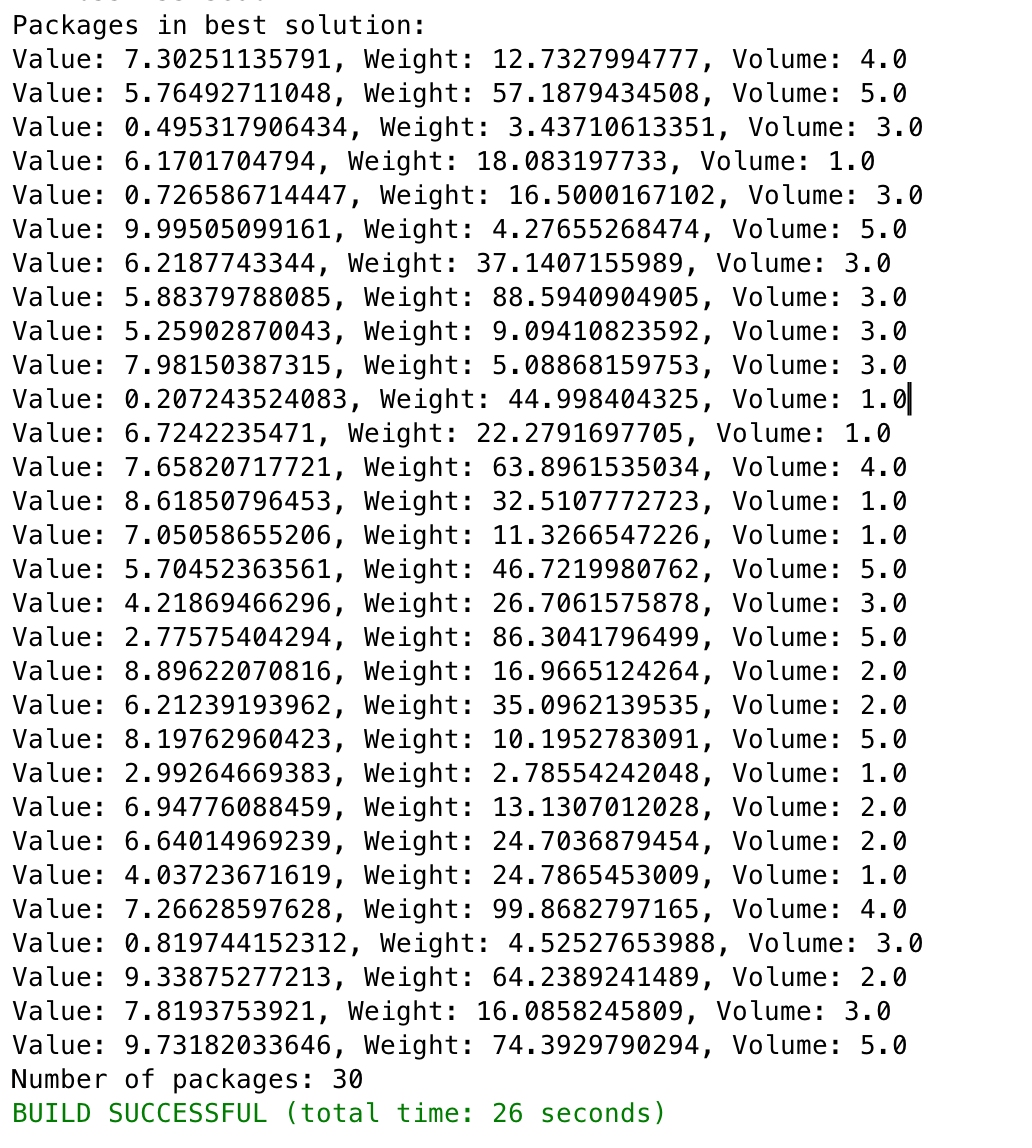
\includegraphics[width=1.0\linewidth]{graphics/simple-knapsack-output.png}
\caption{Output of a knapsack run with just a weight constraint (the volume output is just visible in general).}\label{fig:simple-knapsack-output}
 \end{figure}

In \autoref{fig:pso-knapsack} you can see the plots of three different runs of the algorithm. For us it seems like the different values for c1 and c2 do not make a big difference in the outcome of the algorithm, although this is just a not very scientific observation based on the runs we made by hand.

 \begin{figure}[!htbp]
 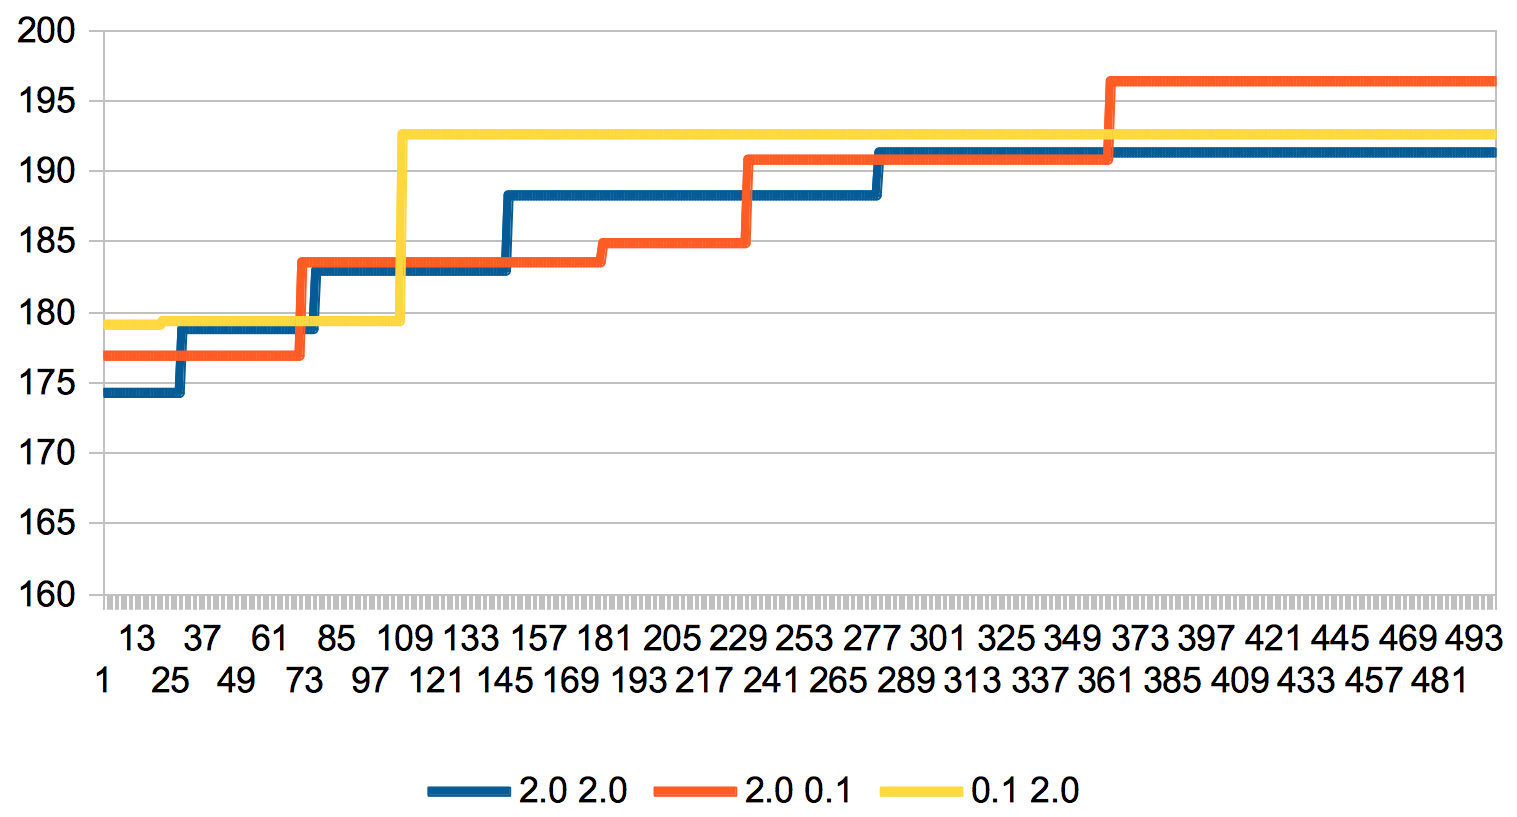
\includegraphics[width=1.0\linewidth]{graphics/pso-knapsack.png}
\caption{Plot of three different Knapsack Problem runs.}\label{fig:pso-knapsack}
 \end{figure}

\section{Task 3 -- Multiple Constraints Knapsack Problem}

The addition of another constraint to the knapsack problem wasn't very difficult for us. As you can see in \autoref{lst:2nd-constraint} we just needed to add another check for the \textit{VOLUME\_LIMIT} instead of just the \textit{WEIGHT\_LIMIT}. This could probably be solved more cleanly, so that future additions of constraints could be added easier, but was sufficient for now.


\begin{figure}
\caption{Adding another constraint to the knapsack problem.}
\label{lst:2nd-constraint}
\begin{lstlisting}
while (weightSum < WEIGHT_LIMIT && volumeSum < VOLUME_LIMIT) {
  selectedPackage = packages.get(this.random.nextInt(packages.size()));
    double newSum = weightSum + selectedPackage.getWeight();
    double newVolumeSum = volumeSum + selectedPackage.getVolume();
    if (!selectedPackages.contains(selectedPackage)) {
      if (newSum <= WEIGHT_LIMIT && newVolumeSum <=VOLUME_LIMIT) {
        selectedPackages.add(selectedPackage);
        valueSum += selectedPackage.getValue();
      }
      weightSum = newSum;
      volumeSum = newVolumeSum;
    }
  }
}
\end{lstlisting}
\end{figure}

\end{document}
